\indent En lo que sigue, mostraremos buenos y malos casos para nuestro algoritmo, y a su vez, daremos el tiempo estimado 
seg\'un la complejidad del algoritmo calculada anteriormente.\\


A continuaci\'on mostraremos un gr\'afico de tiempos comparativo entre distintas familias de casos:\\ 

\vspace*{0.3cm} \vspace*{0.3cm}
  \begin{center}
 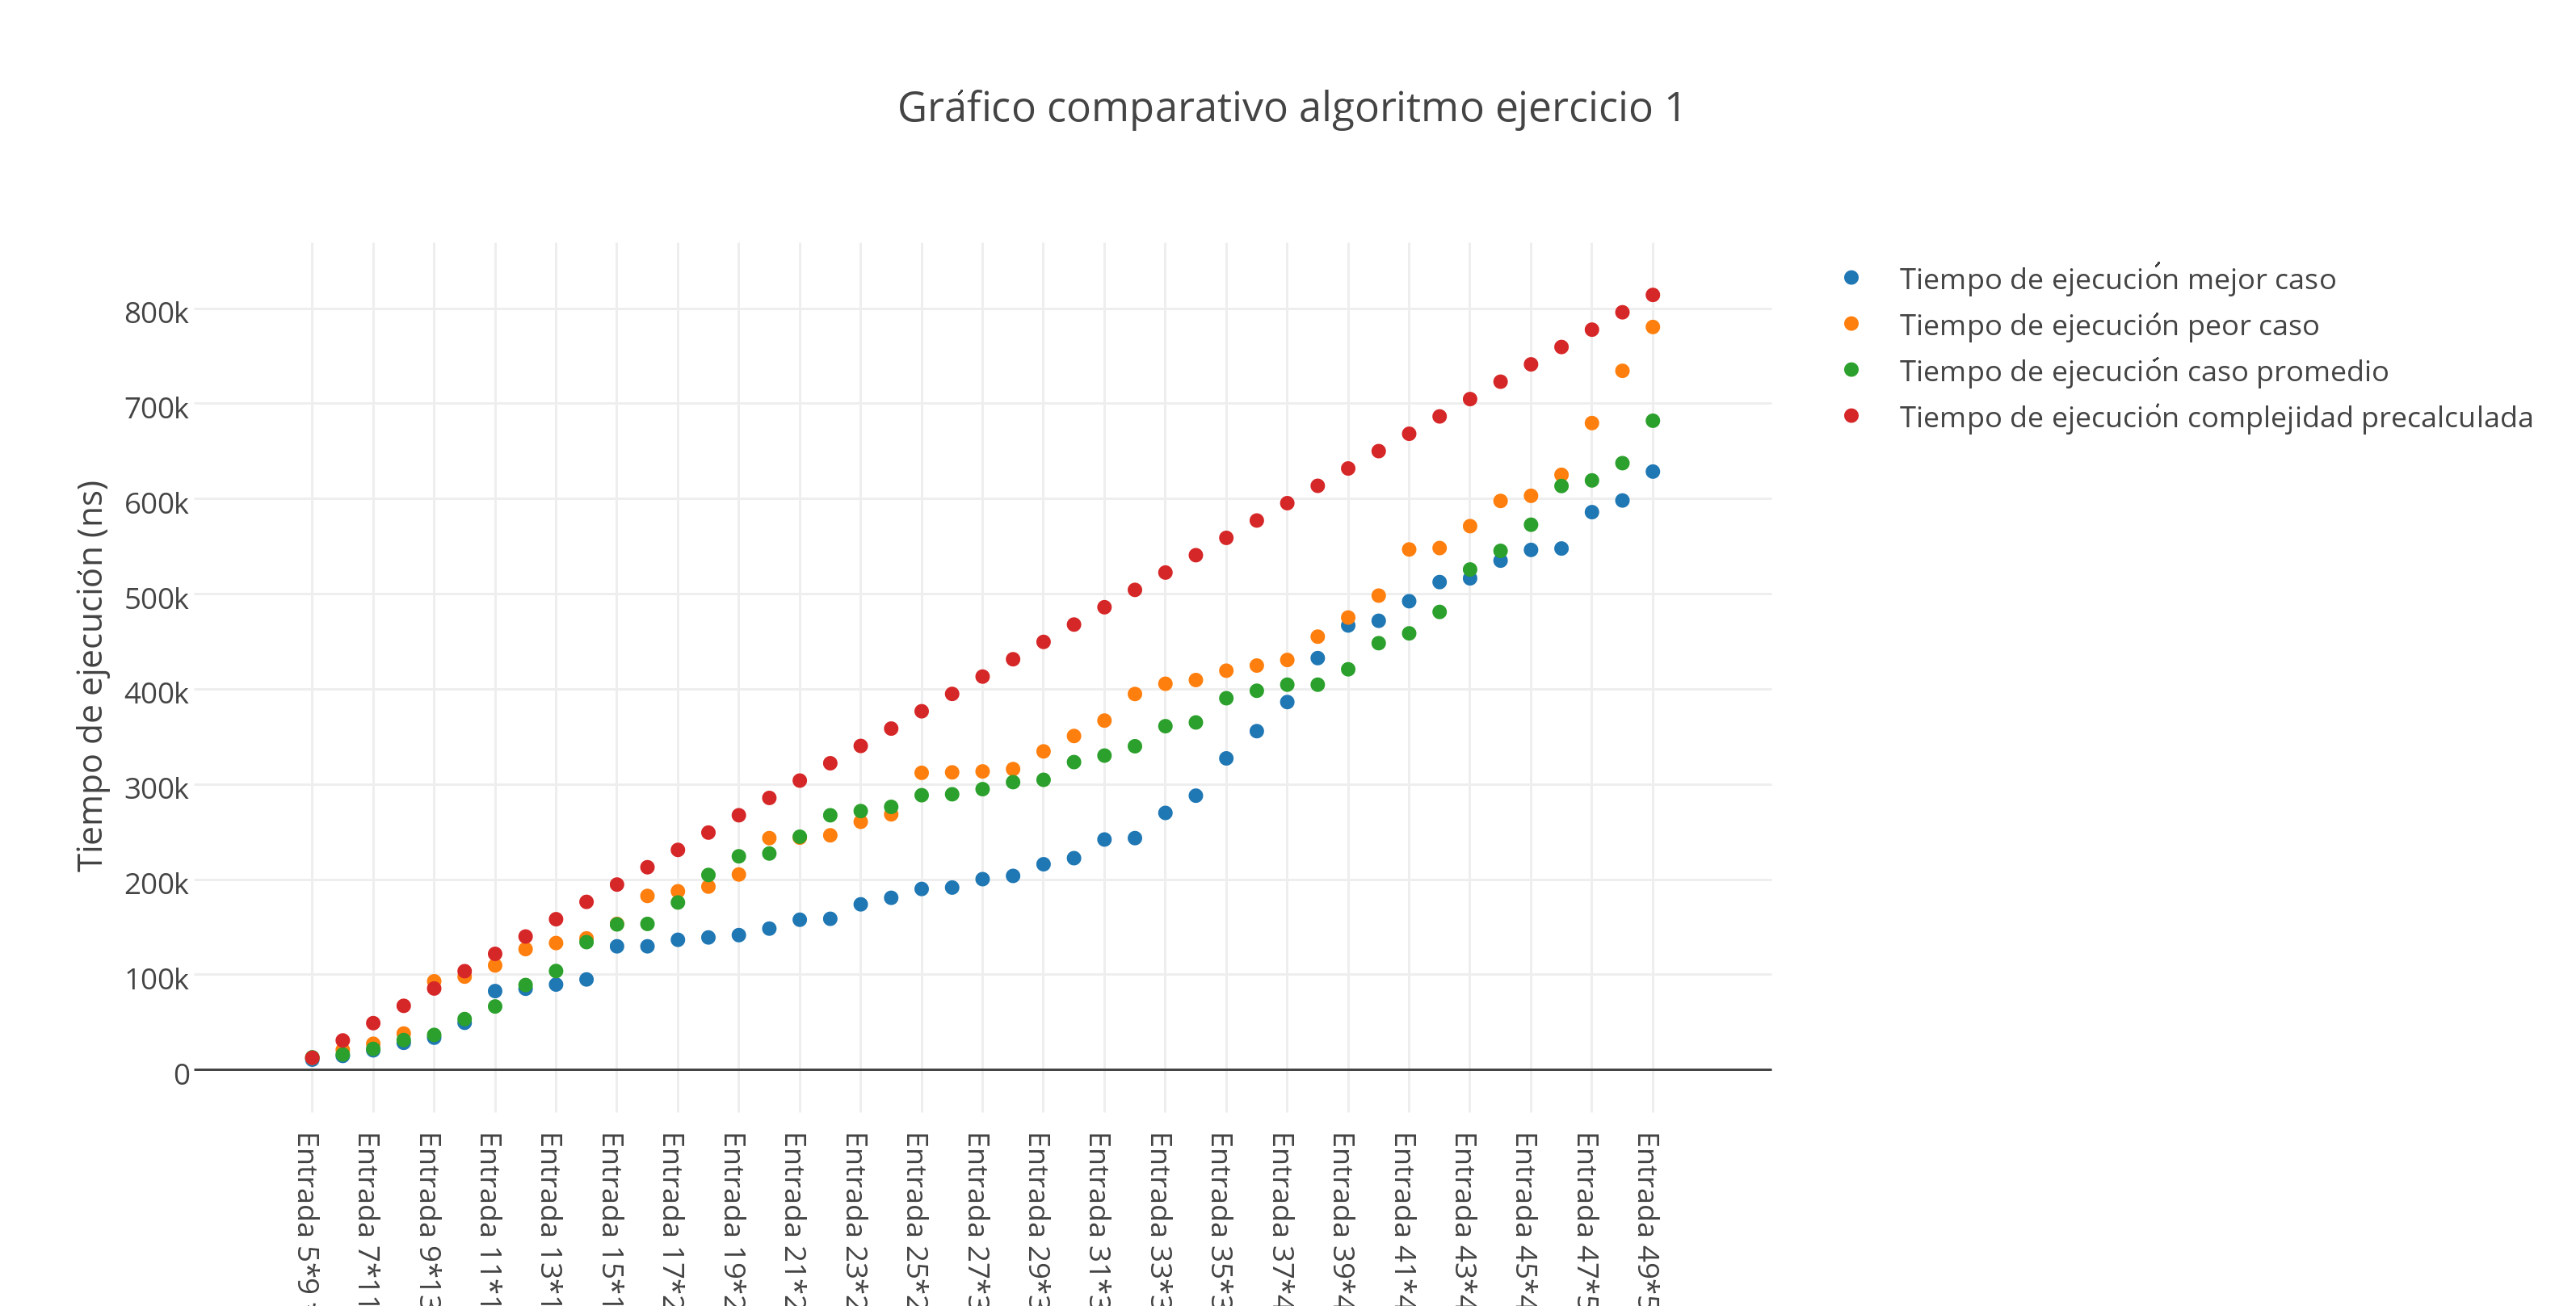
\includegraphics[scale=0.65]{./EJ1/comparativo.png}
 {$Gr$\'a$fico$ \ 1.1 - $Comparativo$}
  \end{center}
  \vspace*{0.3cm}
  
Se puede observar en el gr\'afico, cuatro funciones las cuales representan el tiempo de ejecuci\'on de las familias de casos:\\
\begin{itemize}
\item Sin soluci\'on o con camino m\'inimo inmediato
\item Rompiendo una cantidad de P-1 paredes
\item M\'ultiples caminos a destino posibles
\end{itemize}


Como se observa en el gr\'afico la funci\'on representativa de la flia n\'umero 1, presenta una mejor performance en relaci\'on a las otras. Esto se debe a que en el primer paso no puede salir por ningun camino posible, o su adyacente es el nodo destino por lo tanto chequea solo los nodos adyacentes del origen y finaliza su ejecuci\'on.


El grafo que representa lo dicho ser\'ia el siguiente:\\

\vspace*{0.3cm} \vspace*{0.3cm}
  \begin{center}
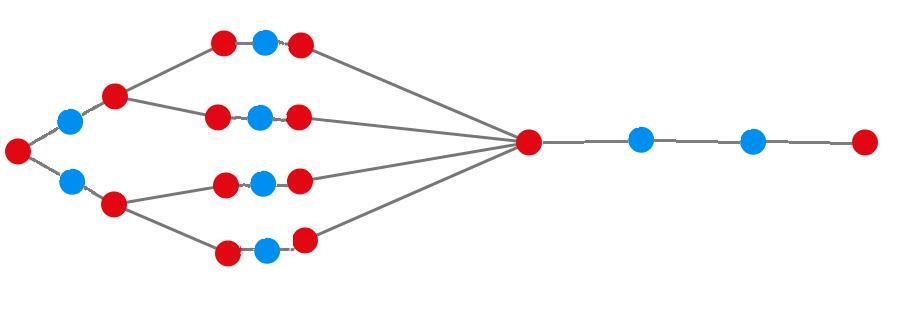
\includegraphics[scale=0.65]{./EJ1/ej1grafomejorcaso.jpeg}
{$Ejemplo Grafo$ \ G1.1 - $Mejor$ $Caso$}
  \end{center}
  \vspace*{0.3cm}


Para una mayor observaci\'on desarrollamos el siguiente gr\'afico con las instancias:\\

\vspace*{0.3cm} \vspace*{0.3cm}
  \begin{center}
 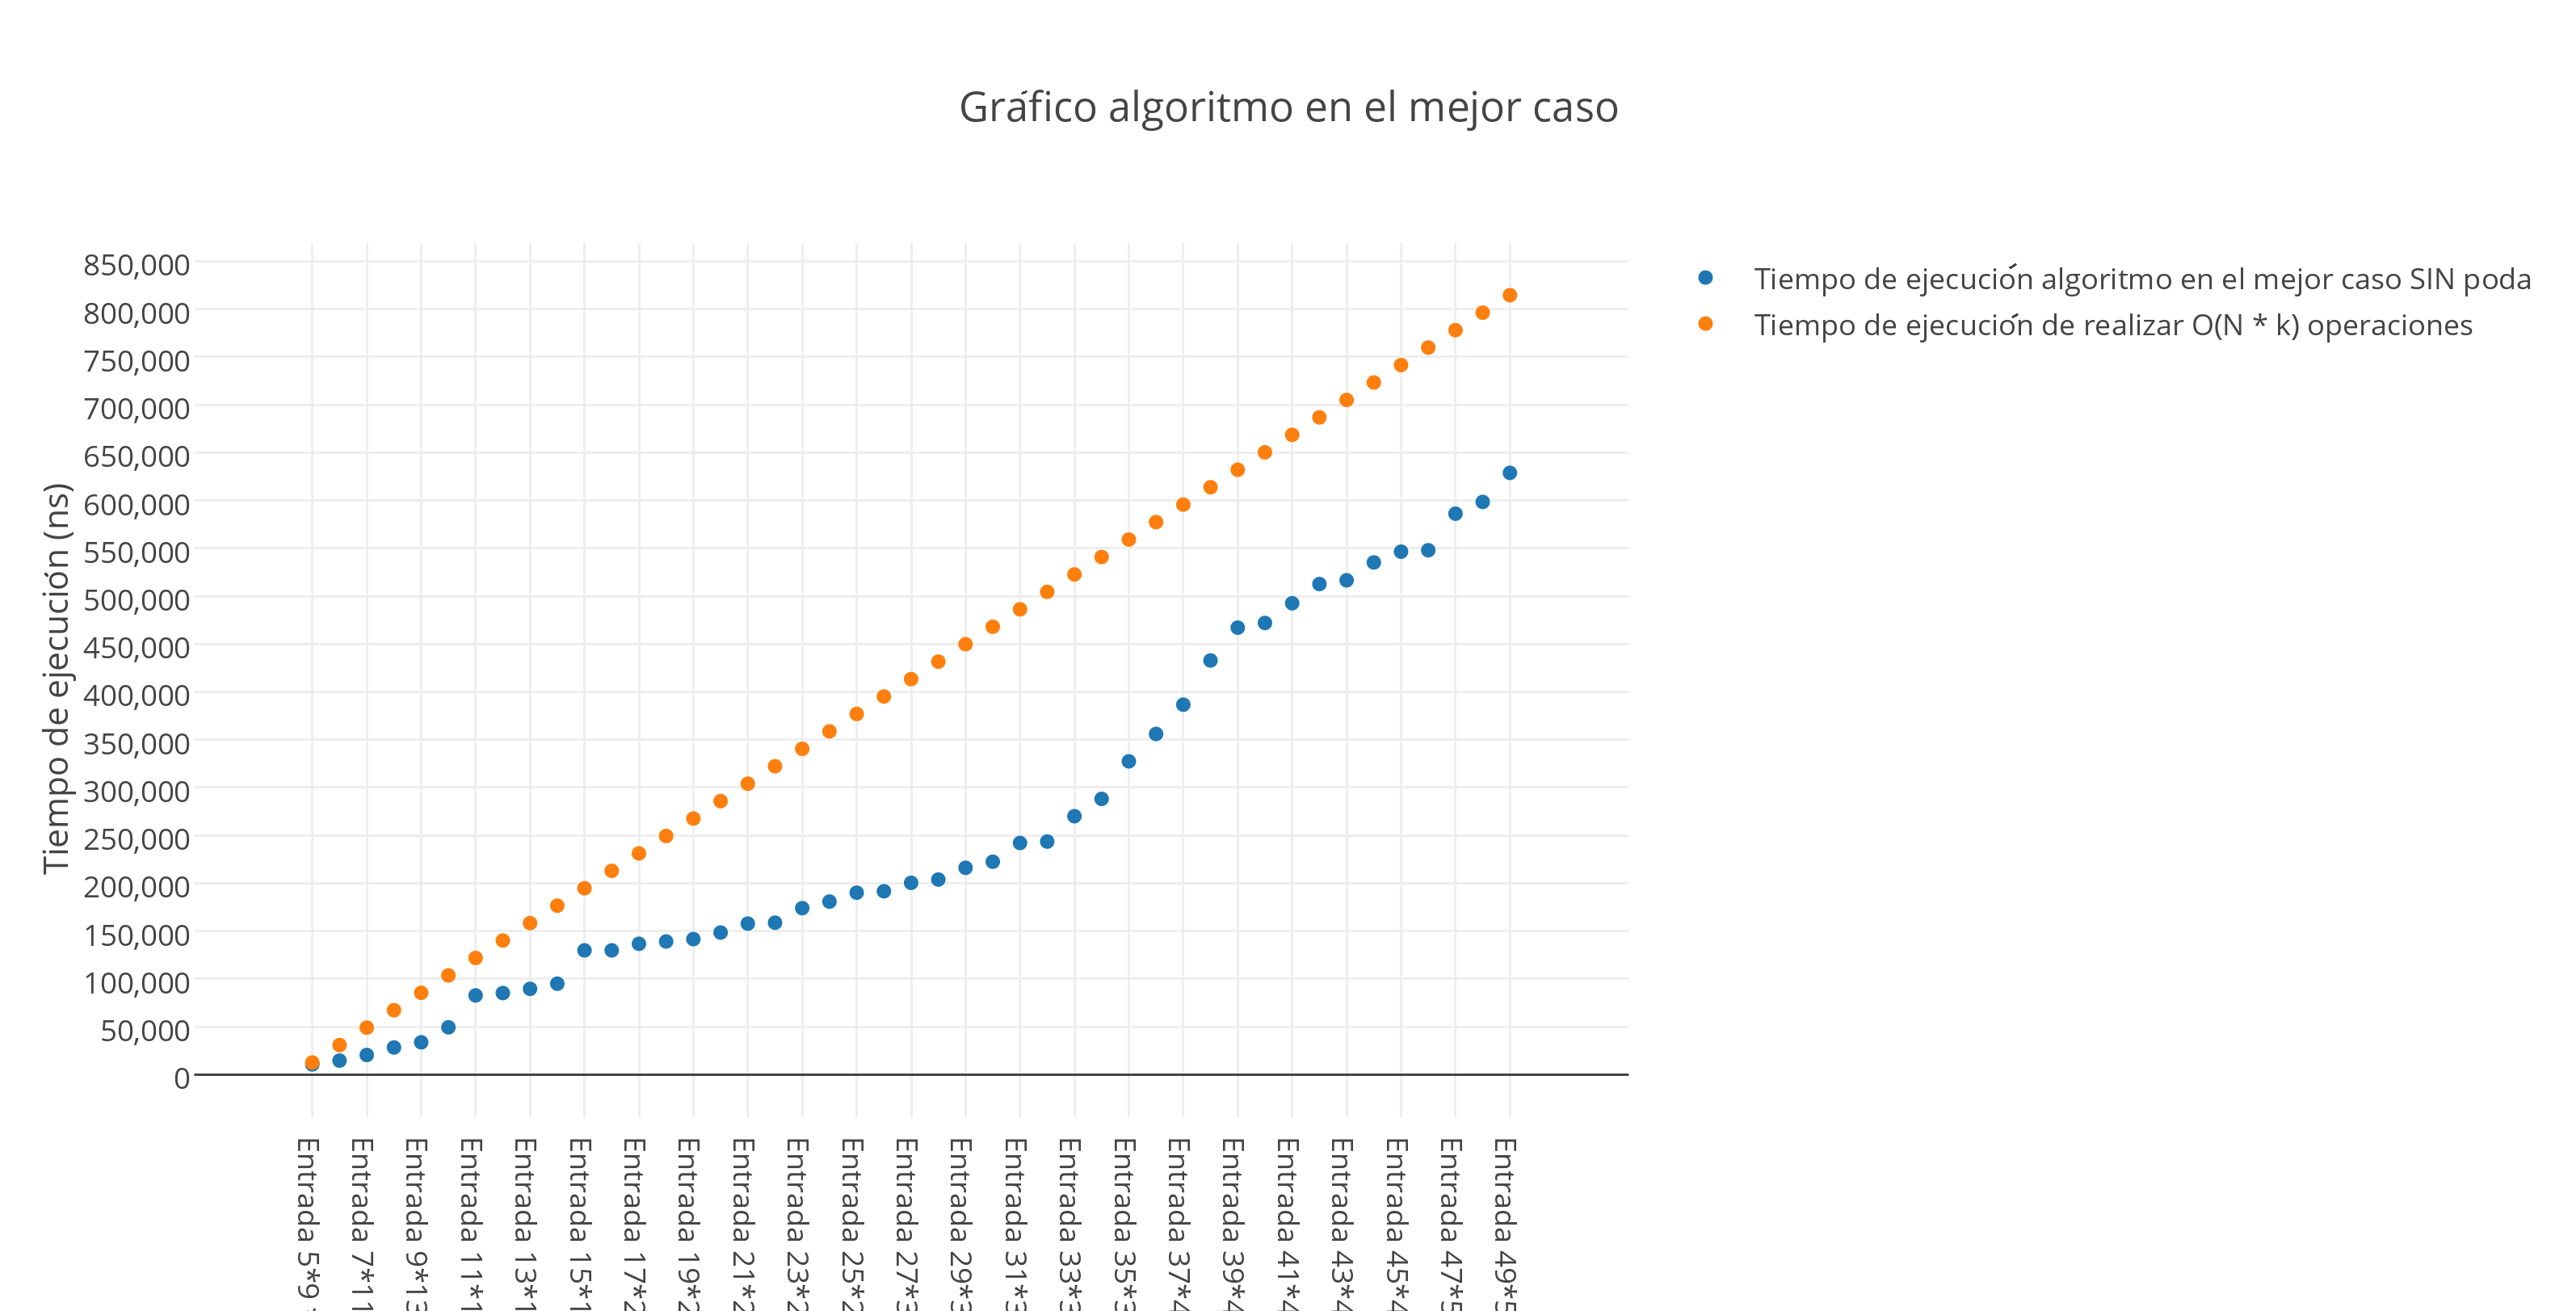
\includegraphics[scale=0.65]{./EJ1/mejorcaso.png}
 {$Gr$\'a$fico$ \ 1.1 - $Mejor$ $Caso$}
  \end{center}
  \vspace*{0.3cm}

Como la complejidad que calculamos se basa en la cantidad de nodos posibles que puede haber multiplicado por las paredes contrastaremos nuestras mediciones con los valores de N (F * C) $\ast$ P .\\

\vspace*{0.3cm} \vspace*{0.3cm}
  \begin{center}
 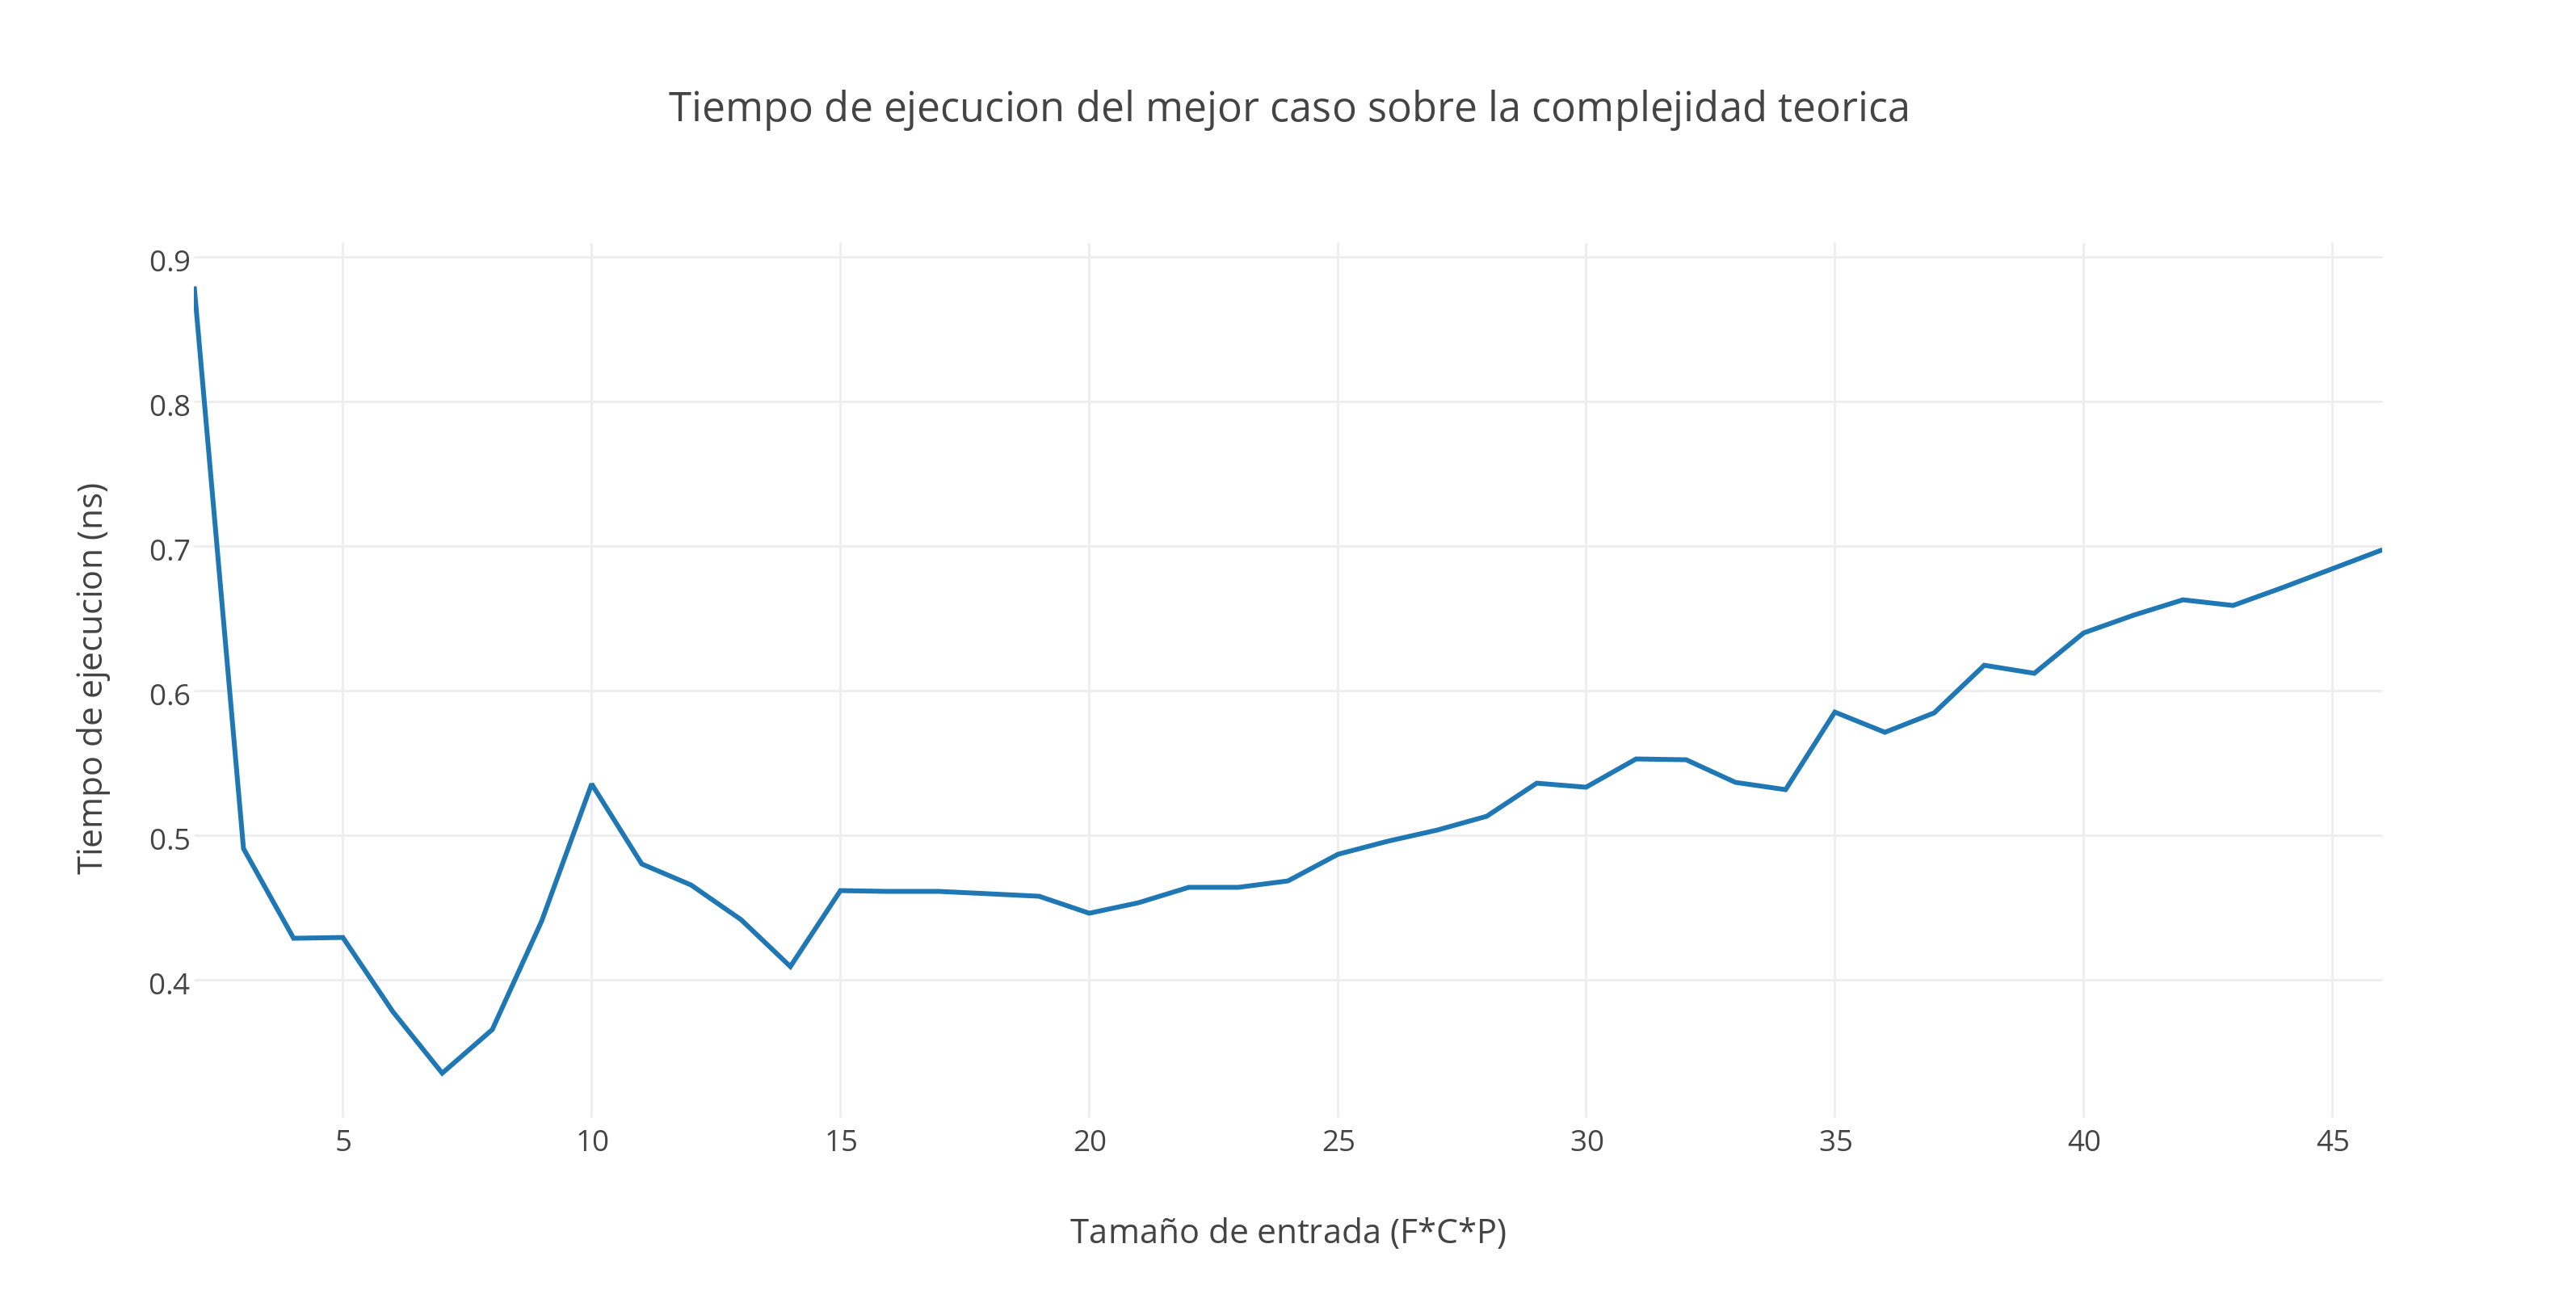
\includegraphics[scale=0.65]{./EJ1/mejorcaso1.png}
 {$Gr$\'a$fico$ \ 1.3 - $Mejor$ $Caso$}
  \end{center}
  \vspace*{0.3cm}

 Para obtener dichas instancias nos resulto prudente realizar aproximadamente unas 20 corridas con el mismo input y sacar el promedio de estas 20 corridas para cada instancia para obtener resultados m\'as consisos.\\ 



Luego, uno de los peores casos para nuestro algoritmo es en el cual  \textbf{se debe recorrer todos los posibles caminos ya que son todos exactamente iguales}, esto se da as\'i ya que nuestro algoritmo chequea todos los caminos posibles y como todos pueden ser soluci\'on posible avanza por todos y llega al final del laberinto con el mismo valor en todos los posibles caminos\\

\vspace*{0.3cm} \vspace*{0.3cm}
  \begin{center}
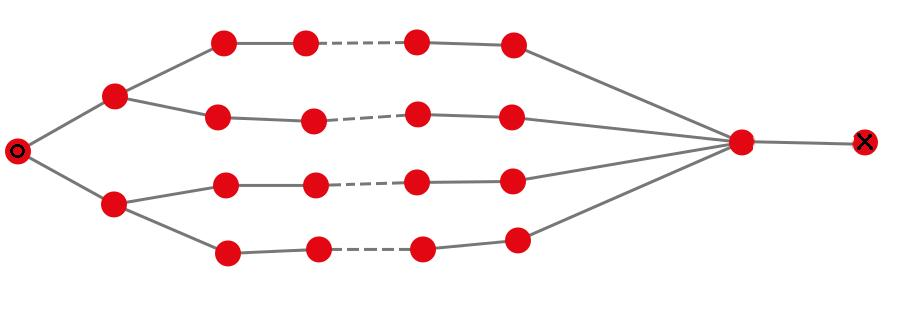
\includegraphics[scale=0.65]{./EJ1/ej1grafopeorcaso.jpeg}
{$Ejemplo Grafo$ \ G1.2 - $Peor$ $Caso$}
  \end{center}
  \vspace*{0.3cm}

Para este grafo realizamos las respectivas mediciones las cuales arrojaron los siguientes resultados:\\


\vspace*{0.3cm} \vspace*{0.3cm}
  \begin{center}
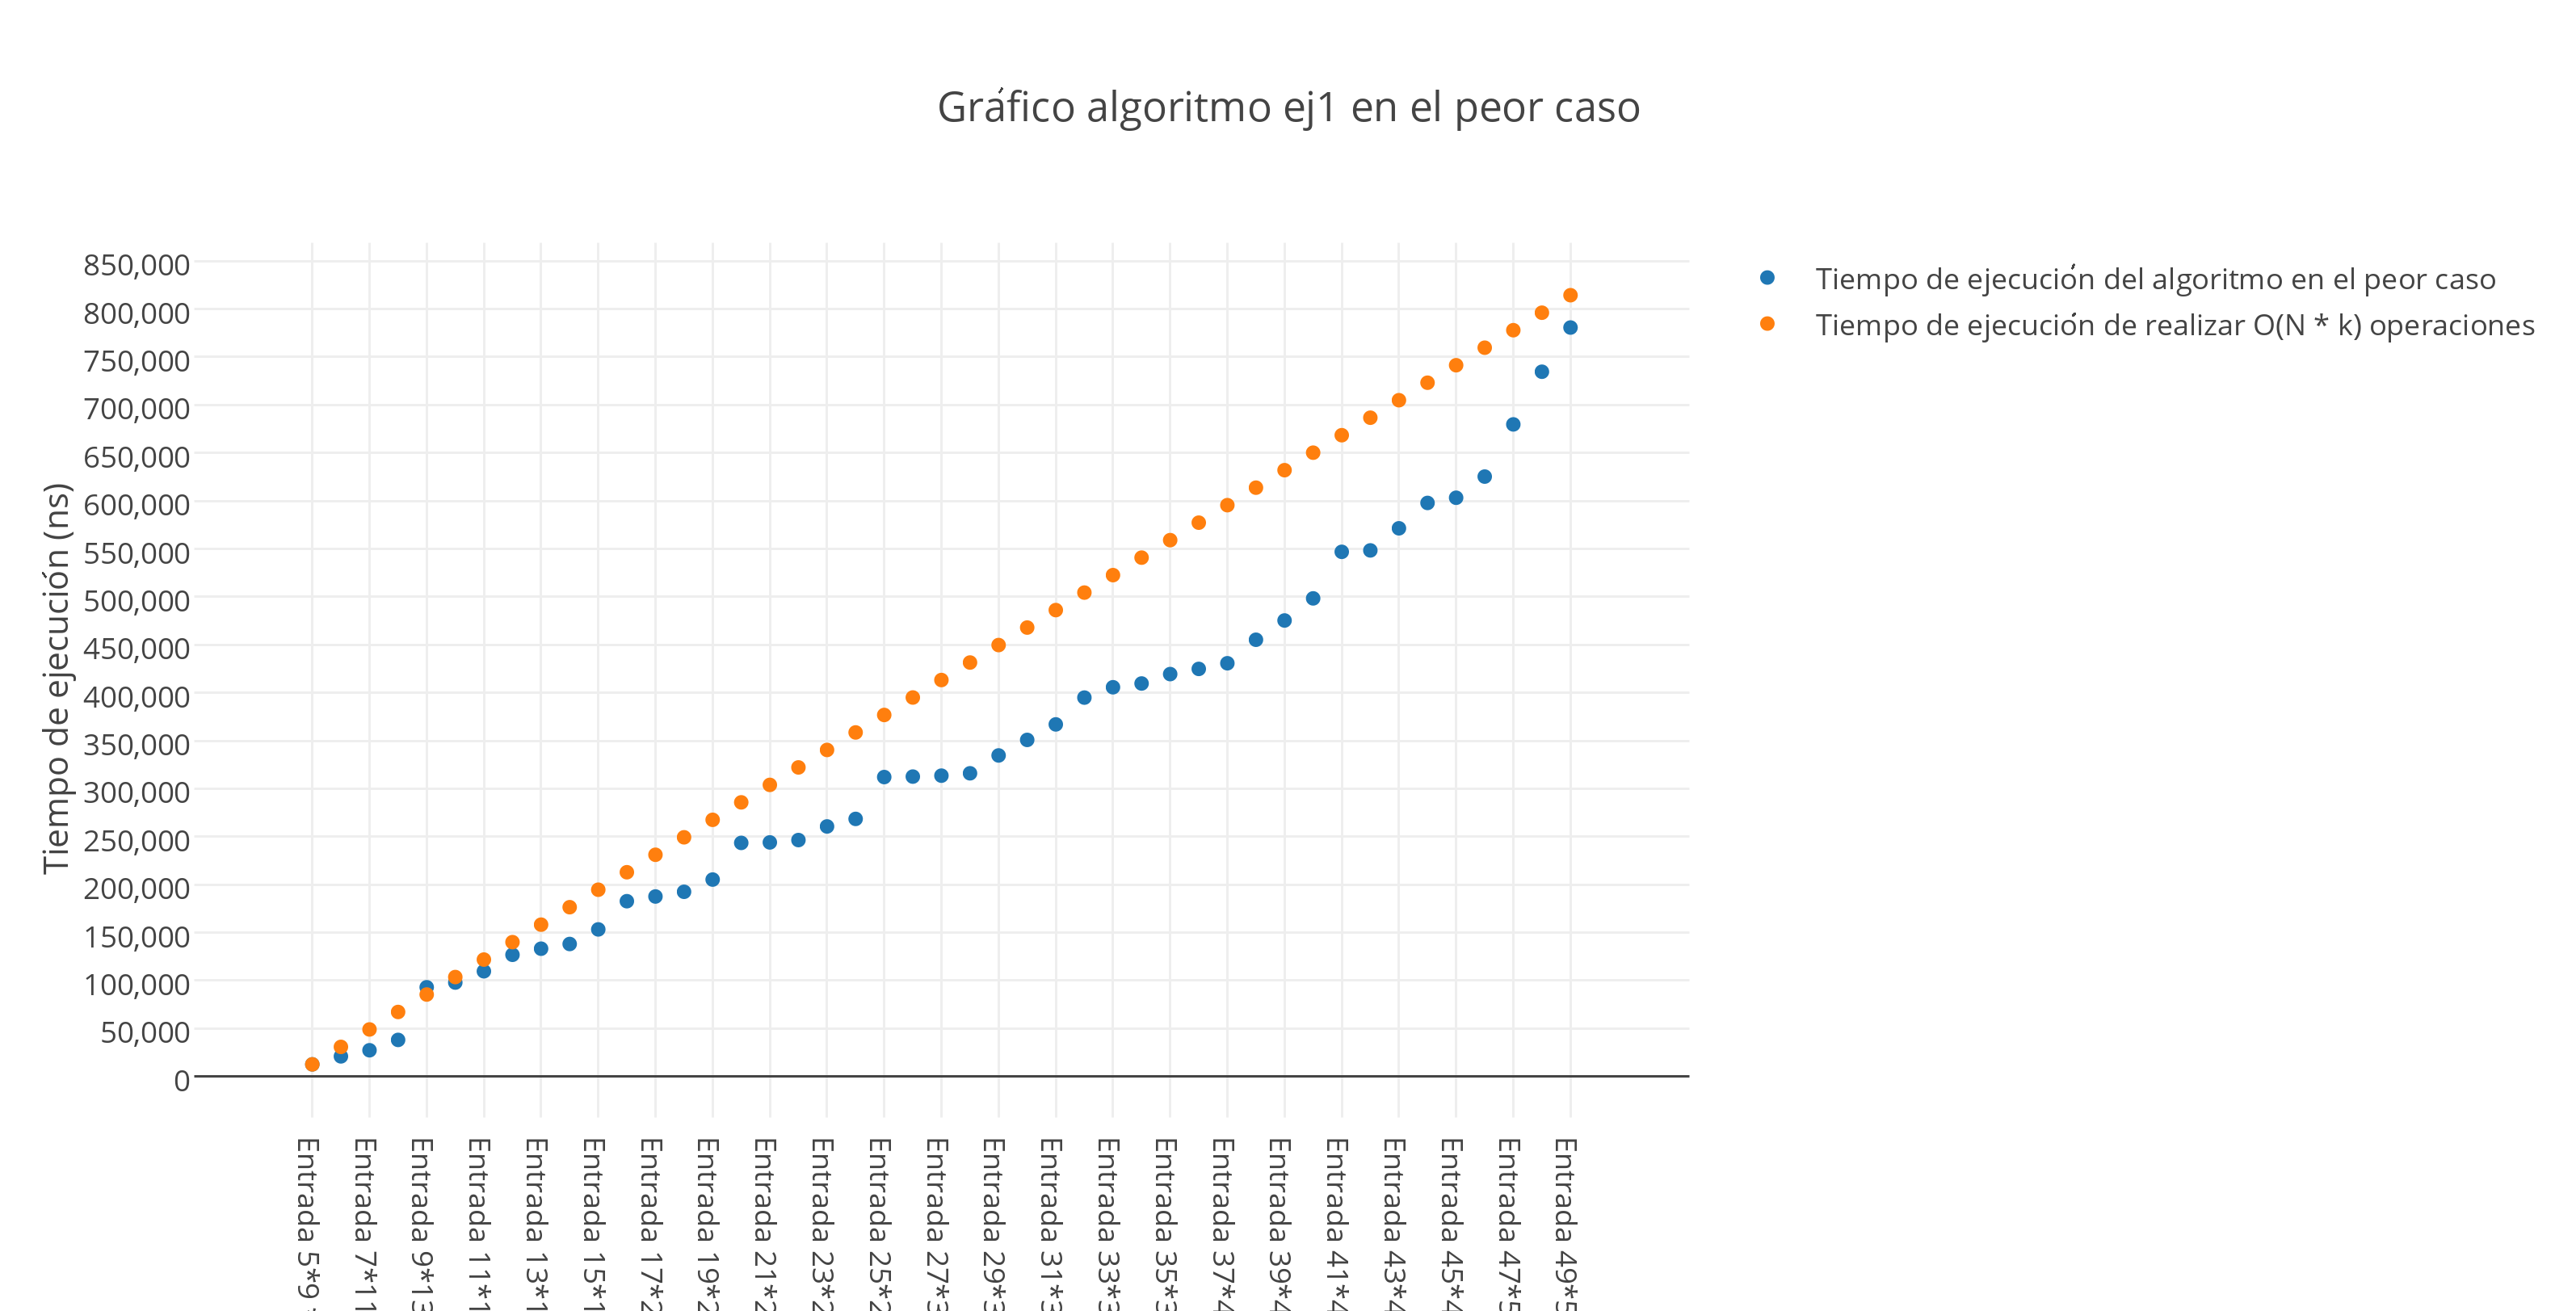
\includegraphics[scale=0.65]{./EJ1/peorcaso.png}
{$Gr$\'a$fico$ \ 1.7 - $Peor$ $Caso$}
  \end{center}
  \vspace*{0.3cm}


\vspace*{0.3cm} \vspace*{0.3cm}
  \begin{center}
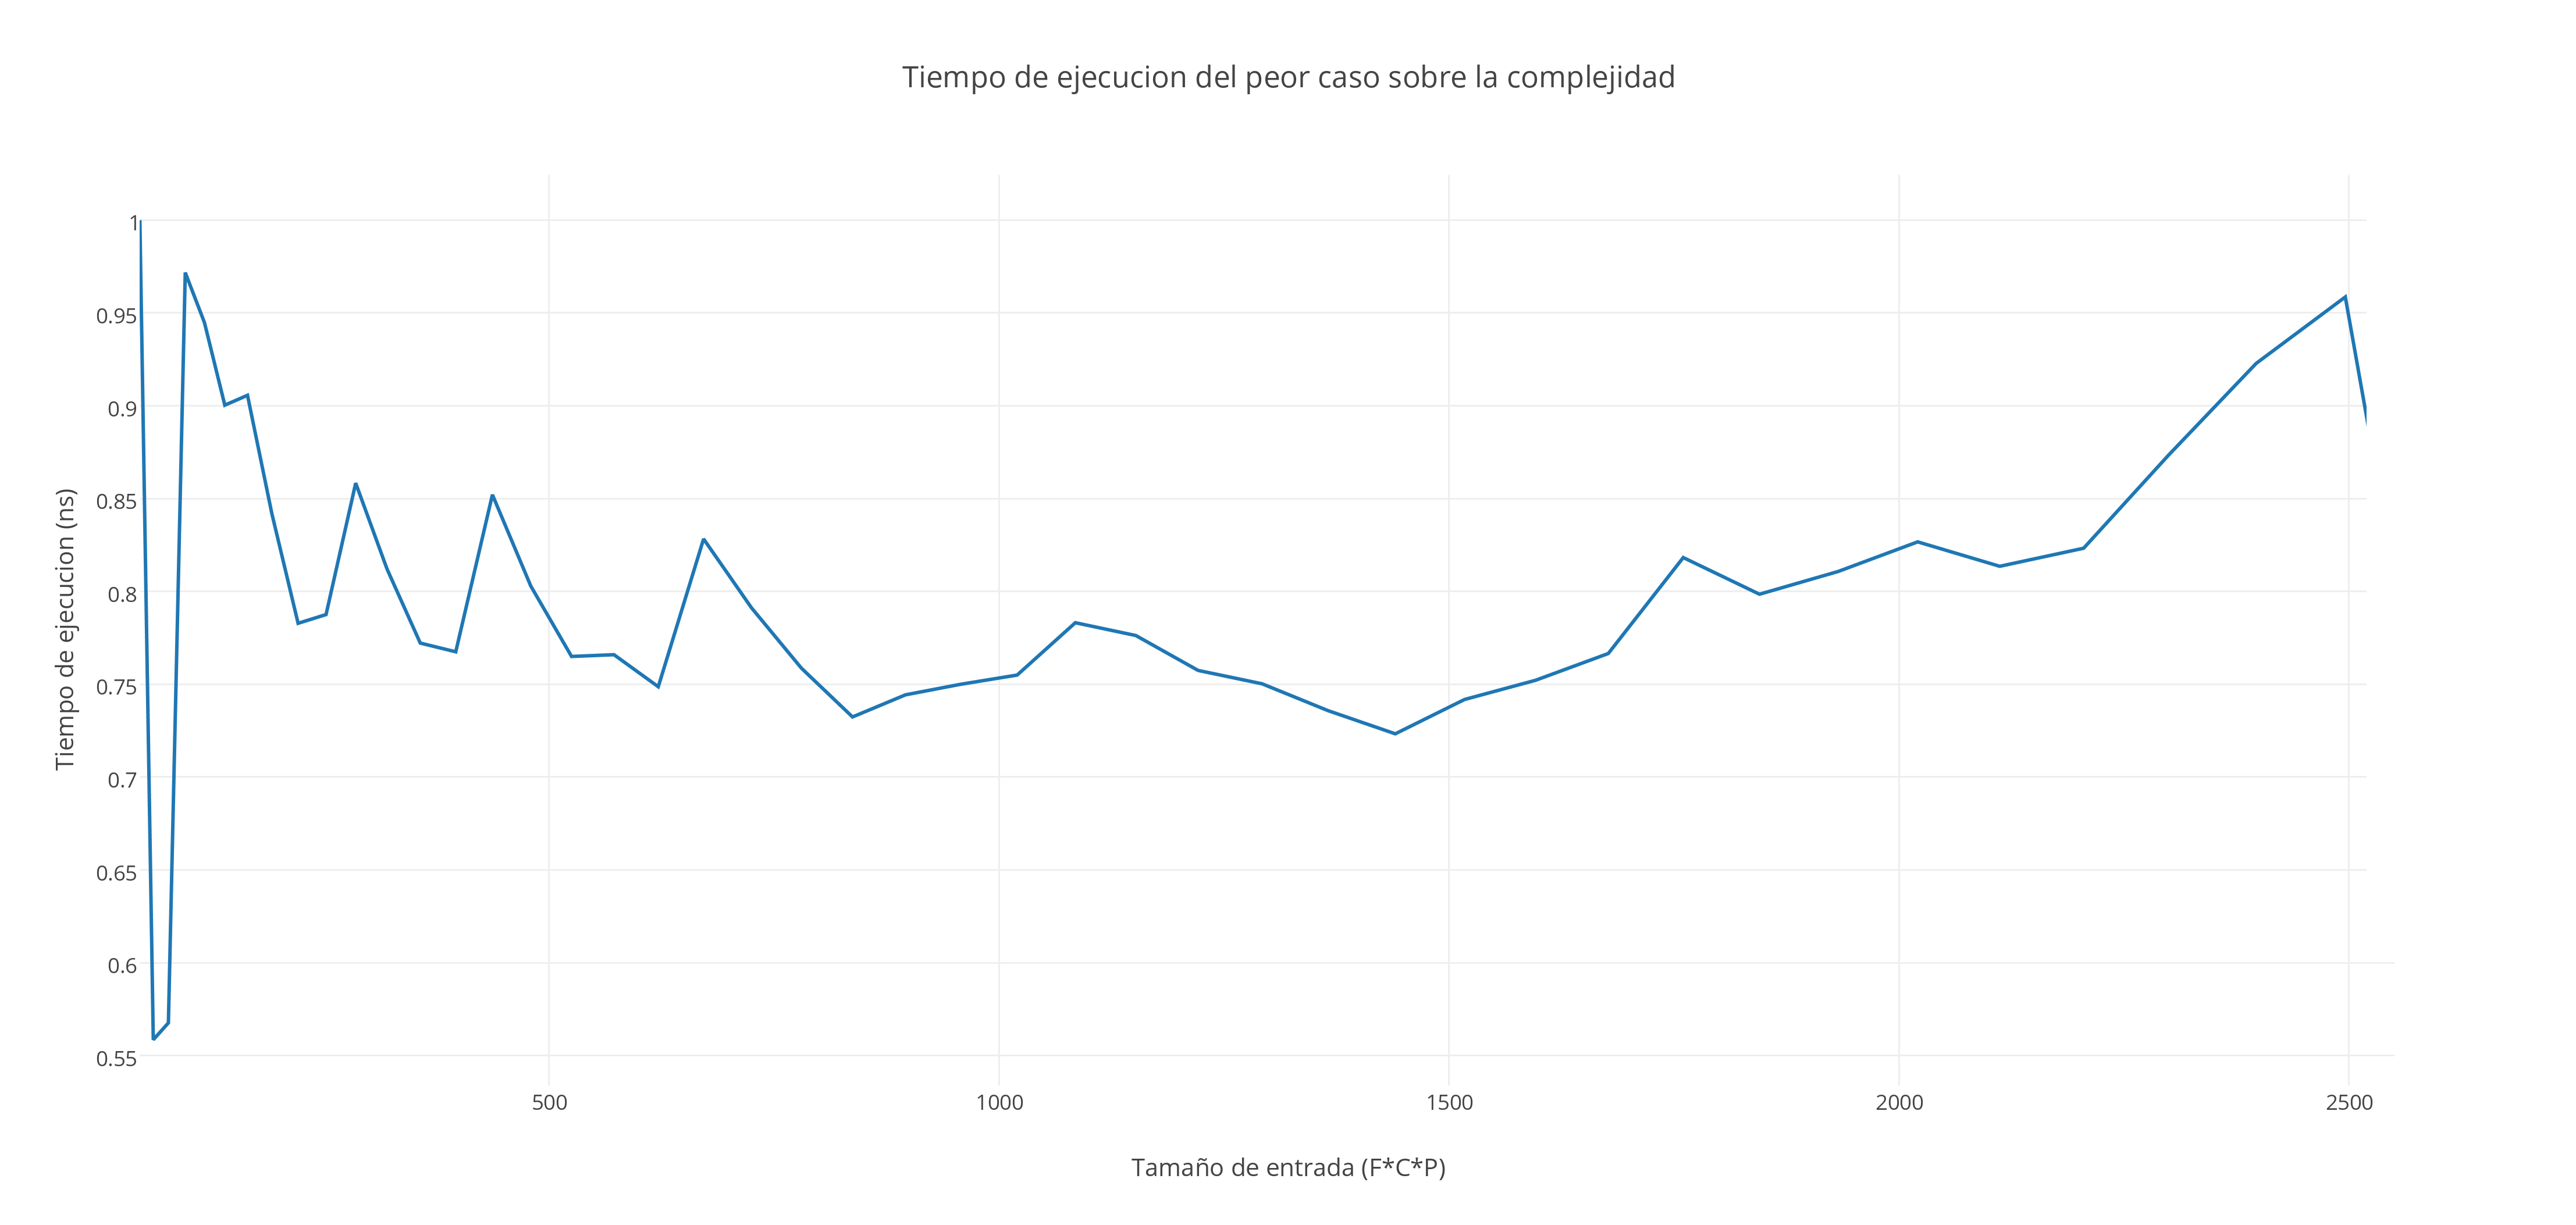
\includegraphics[scale=0.65]{./EJ1/peorcaso1.png}
{$Gr$\'a$fico$ \ 1.7 - $Peor$ $Caso$}
  \end{center}
  \vspace*{0.3cm}

 Para obtener dichas instancias nos resulto prudente realizar aproximadamente unas 20 corridas con el mismo input y sacar el promedio de estas 20 corridas para cada instancia para obtener resultados m\'as consisos.\\ 

Podemos observar en la figura 1.5 como la funci\'on resultante de nuestro algoritmo en el peor caso se mantiene por debajo de la funci\'on final del tiempo de realizar O(N * k) operaciones lo cual fue la complejidad precalculada.\\

Por \'ultimo mostraremos un gr\'afico comparativo con el mejor, el peor y el caso promedio contra la complejidad precalculada .\\

  
  \vspace*{0.3cm} \vspace*{0.3cm}
  \begin{center}
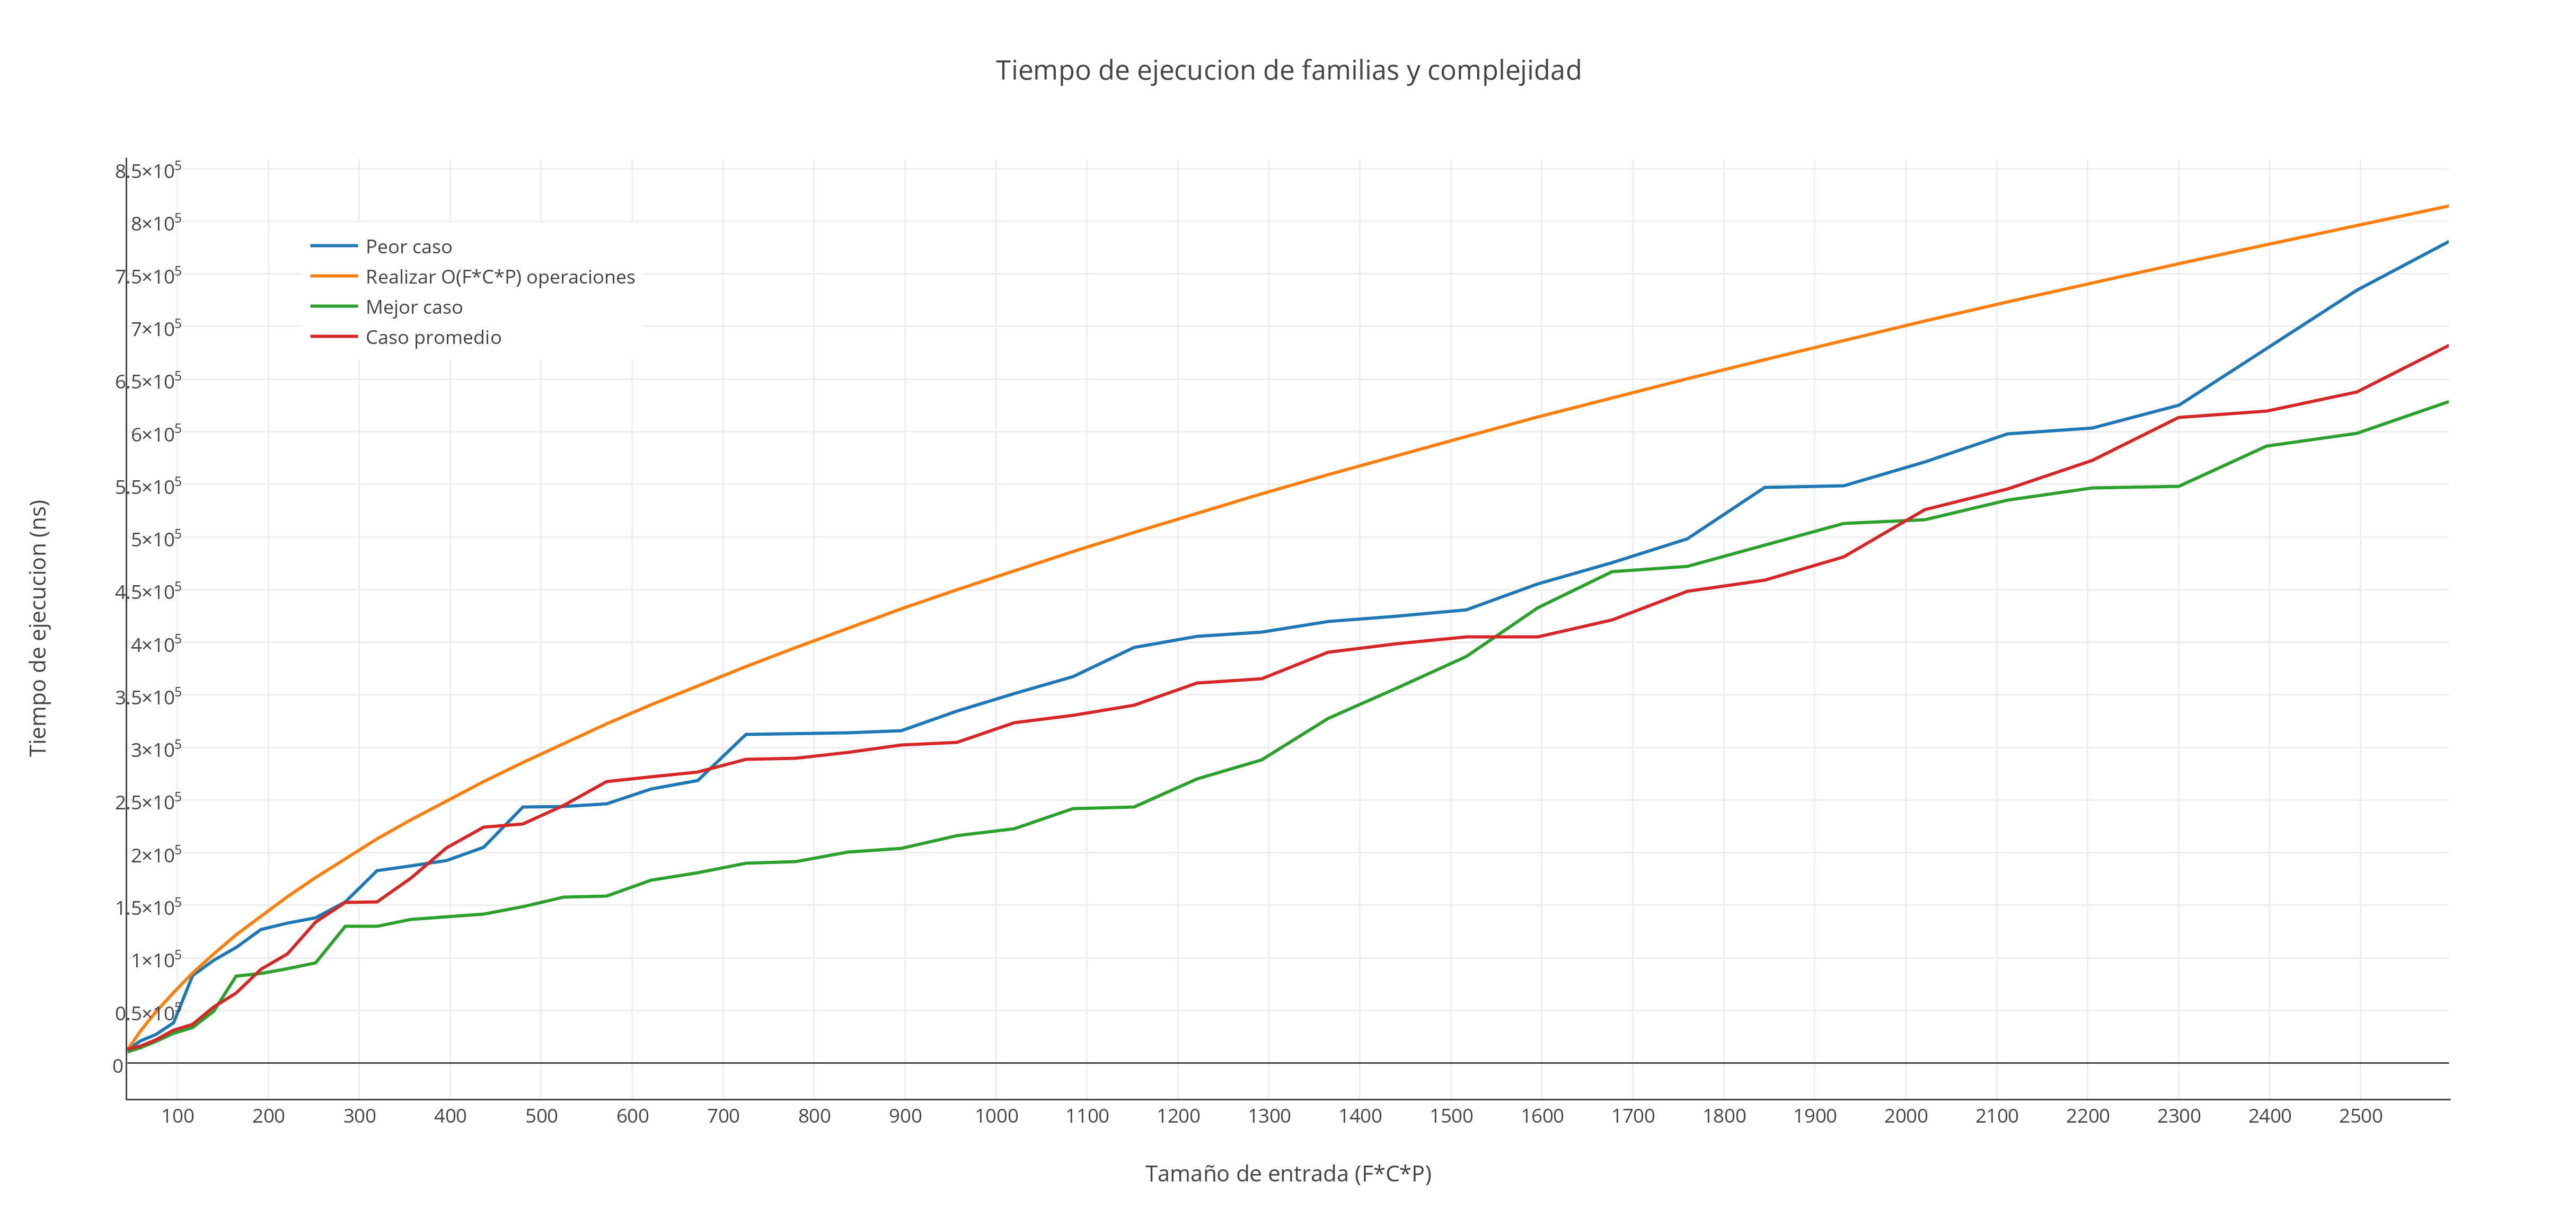
\includegraphics[scale=0.65]{./EJ1/comparativo1.png}
{$Gr$\'a$fico$ \ 1.10 - $Comparativo$}
  \end{center}
  \vspace*{0.3cm}


Luego de lo mostrado, podemos ver que ya sea en el peor caso nuestro algoritmo en funci\'on al tiempo de ejecuci\'on queda asintotizado por debajo de la funci\'on del tiempo de la complejidad .